%%%%%%%%%%%%%%%%%%%%%%%%%%%%%%%%%%%%%%%%%%%%%%%%%%%%%%%%%%%%%%%%%%%%%%%%%%%%%%%%%%
%%% Introduction
%%%
%%% What are we trying to get done?
%%% How to we tackle the problem?
%%% Why did we use this approach?
%%% Why did we use this platform?
%%%
%%% Section 1 : Concept and Motivation
%%% Section 2 : Platform Overview
%%% Section 3 : Problem Domain
%%% Section 4 : Implemented Components
%%%		SubSection 4.1 : Navigation
%%% 	SubSection 4.2 : Crawlspace Detector	
%%%		SubSection 4.3 : Crawl Gait
%%% Section 5 : Thesis Structure
%%%
%%%%%%%%%%%%%%%%%%%%%%%%%%%%%%%%%%%%%%%%%%%%%%%%%%%%%%%%%%%%%%%%%%%%%%%%%%%%%%%%%%
\chapter{Introduction} \label{ch::introduction}

\section{Concept and Motivation}
% We are trying to make things that help the robot get from A to B.
% The problem of getting the robot from A to B looks like this: stuff, stuff, stuff.
A common task for robotic systems is for a mobile platform to transport itself from one location to another
in the presence of environmental obstacles. Within this general task there are many subproblems. The system
must have some sort of awareness of the destination objective and usually some notion of where it is relative
to that destination. The destination location and the location of the robot can be encoded in a map that
the mobile platform or some off board system is responsible for maintaining. Within the environment there may 
be obstacles that prevent the robot from moving through that space which can also be encoded into the map. 
Given these notions of robot, goal, and obstacle locations often an initial path is planned to allow the robot
to reach the goal location. In addition to these higher level concepts, the robot must have a scheme by which it
transports itself through the environment be rolling, walking, flying and controls for each of those methods.
Solutions to these subproblems, map building, robot localization, obstacle localization,
path planning, locomoting and others work together to accomplish the overall goal. 
Each of these subproblems can be expanded upon and this thesis works on three of these components: 
local navigation, obstacle detection and characterization, and gaiting. Used to work on these problems
was the Nao Humanoid Platform by Aldebaran Robotics.

\begin{figure}[h!]
	\centering
	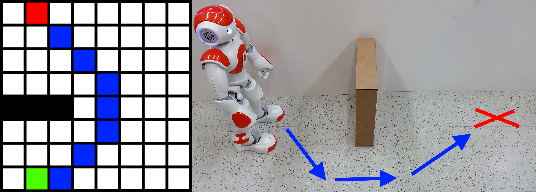
\includegraphics{nao_with_obstacle_and_map1.png}
	\caption
	{Example illustration of the Nao humanoid robot in an environment with an obstacle. The red X represents a goal
		location with the blue arrows showing an possible path. On the left side is one possible representation
		of the environment as a 2D grid.}
	\label{fig:nao_with_map1}
\end{figure}


\section{Platform Overview}
% As a medium we worked with the Nao. The Nao is good because this: stuff, stuff, stuff.
The broader task of moving an agent from one location to another is applicable to a wide range of robots but
each platform will have details that change the scope of the problem and the method used to approach it.
The three problems focused on (local navigation, obstacle detection, and gaiting) for a flying robot with 
a global camera system will require different solutions than a wheeled robot with only rangefinders.
For this thesis, the Nao H25 V4 Humanoid Platform by Aldebaran Robotics was chosen to act as the mobile base. 
With the future goal of having robots interact in human environments, humanoid platforms have become an active
area of research as they are physically compatible with such environments. 
While Nao is a 1.9 ft tall humanoid weighing 9.5 lbs and therefore only an appropriate analog for a young human toddler,
the humanoid format is of primary importance to algorithmic development.
with 25 degrees of freedom including two legs, two arms, and two grippers. 
Figure~\ref{fig:nao_diagram1} shows a cursory illustration of the humanoid configuration.
This lightweight but capable configuration enables research into mobile manipulation, humanoid gaiting, and terrain adaptation
without the need for specialized support equipment such as belays or dedicated experimentation areas as the
robot is safe for humans to interact with.

\begin{figure}
	\centering
	\includegraphics[width=0.4\textwidth]{nao_coronal_highlighted2.png}
	\caption
	{Coronal view of the Nao humanoid with a few pertinent features highlighted. }
	\label{fig:nao_diagram1}
\end{figure}

The robot comes with a suite of sensors including two cameras, two ultrasonic rangefinders, 
a 3-axis accelerometer and 2-axis gyro, foot contact sensors, and angular position encoders on every joint.
Such a complement of sensors aids the robot in creating an estimate of a number of variables including 
the robot state and environment characteristics. 
Nao has a built-in WiFi radio and 1.6 GHz Intel Atom processor running a version of the Linux operating system 
allowing the robot to be programmed in C++ or Python using standard libraries that can be remotely uploaded.
These features allow the use of a wide variety of tools when constructing new algorithms and for program
iteration to happen at a rapid pace.

With all of these features the Nao makes for a convenient platform for the development of mobile robot algorithms.

% Then we stuck a Hokuyo laser on the Nao and used that for navigation. Why was this a good idea?
To augment the sensor suite, a Hokuyo URG-04LX-UG01 Scanning Laser Rangefinder (Lidar) was mounted to the Nao and
interfaced via a USB connection to the Nao's onboard computer. The sensor has a scanning area of $240^\circ$ with 
an angular resolution of $0.36^\circ$ and a range of 5 meters. It is used to generate a planar point cloud representing
the range to the nearest occlusion at a set of fixed bearing relative to the robot. Lidars are commonly used in mobile
robotics so developing algorithms utilizing them is of practical concern.

\section{Problem Domain}
% Within this, we restrict the problem to this: stuff, stuff, stuff.
The three areas selected for development were local navigation, obstacle detection and characterization, and gaiting.
Each of these is a broad research topic in its own right so the domain of investigation for each problem
must be specified. 

\section{Implemented Components}
% Within this problem well address certain components that add to our problem solving toolbox.
% These are the things we developed: thing 1, thing 2, thing 3.

\subsection{Navigation}
% \subsection{Crawlspace Detector}
% Used the camera data (and gyro) to detect openings using SFM and Lidar to confirm.
\subsection{Crawl Gait}

Many robots that enjoy practical use are not mobile. They are affixed to a table or floor
and do not depend on their environment in order to produce a commanded movement. They 
utilize a motion model that describes how their parts interact with each other to move an
end effector and typically avoid interacting with objects in their environment other than those
they are required to manipulate.
Mobile robots also use a motion model to plan their movements but, in contrast to fixed robots, must interact
with their environment to produce movement. 
While this can be a more challenging problem than motion planning for fixed robots, the use of
the environment to produce motion leads to mobile robots having a richer and more adaptable set of movements.
Aerial and aquatic vehicles push against water or air,
wheeled robots roll over the ground, legged robots walk, run, and crawl.
Not only can mobile robots operate through a wider set of environments than fixed robots, but different
actuation schemes can be employed to produce different movements. Legged robots are a particularly interesting
platform for ground locomotion, as opposed to wheeled platforms, because they are more adaptable
to a wide range of environments by actuating their legs according to a different strategy.
Collectively, the method by which legged robots actuate their legs as a function of time is called 
gaiting. Different gaits produce different characteristics such as the range of
achievable speeds, endurance, terrain adaptability and a host of other things.



% Approaches to solving the problem - CPG actor critic paper
Someone else used a CPG network with an actor-critic scheme to generate a baby gait on a Nao and iCub.

\section{Thesis Structure}
This thesis is organized as follows: 

% Chapter \ref{ch:platform} reviews the Nao Humanoid Platform with Hokoyu Scanning Laser Rangefinder augmentation.
% The navigation system is broken into three parts, 
% Chapter \ref{ch:navigation} discusses the GODZILA algorithm used for local navigation.
% Chapter \ref{ch:detector} discusses SFM for detecting openings that the Nao might crawl under,
% Chapter \ref{ch:crawl_gait} discusses the Projected Profile crawling gait used to perform the crawl.
% Simulations and experimental results are shown in Chapters \ref{ch:simulations} and \ref{ch:results}, 
% while a discussion of the work is given in Chapter \ref{ch:conclusion}.








% Results from this work were published in \cite{our_paper1}.
% And more results were published in newer papers.

